This section describes our system by presenting it in different layers, illustrating the layer that captures data on the top, and interacting with the lower-level layer on the bottom, the data processing layer. The Data Capture Layer components both obtain information from the Data Processing Layerr, such as current medication stored in the database, and information inputted by the user from the Data Capture Layer into the Data Processing Layer.  

\begin{figure}[h!]
	\centering
 	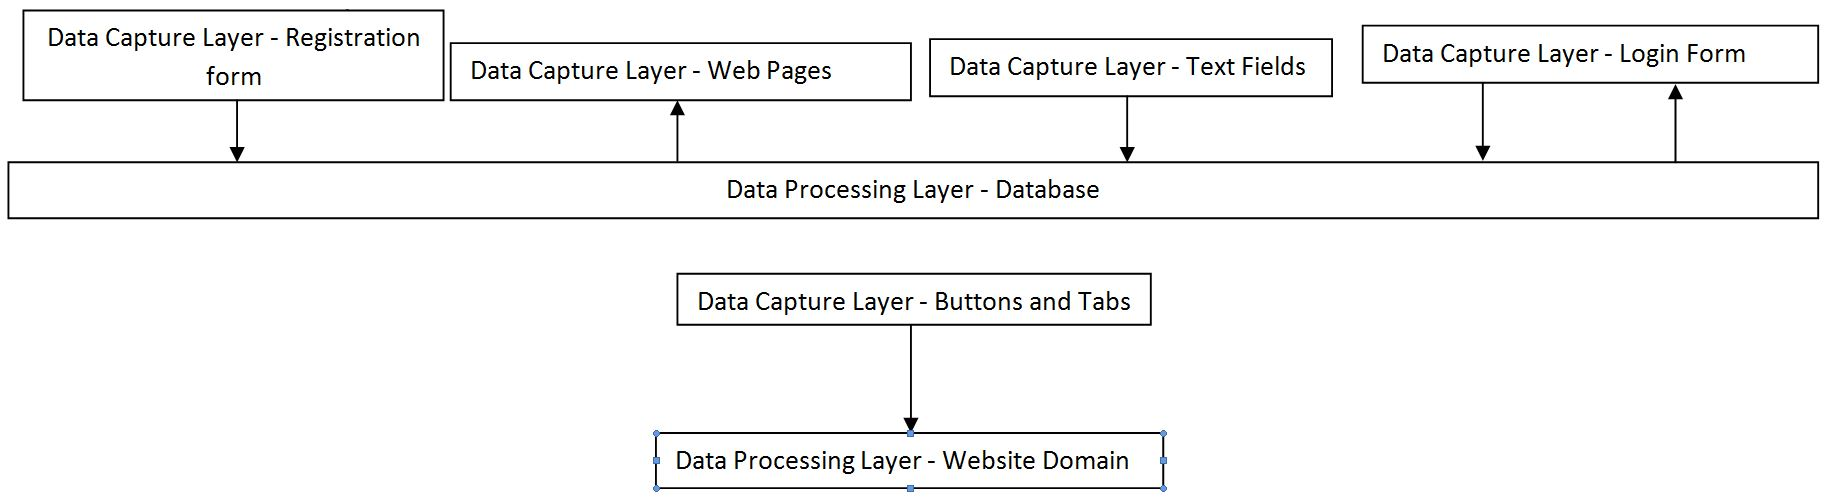
\includegraphics[width=1\textwidth]{images/LayerBlockDiagram2}
 \caption{A simple architectural layer diagram}
\end{figure}

\subsection{Data Capture Layer Description}
 

\subsection{Data Processing Layer}
This layer takes information inputted by the user, such as registration information, and inputs this information in the database. This information is then evaluated when the user tries to login using their credentials, which are their email and password. Upon logging in, the user can input medications on the Medication tab, and this information will be stored in the database. Other information, such as user information, which can be accessed from the Management tab, can be edted, and thus changed in the database. 

\subsection{Layer Z Description}
Each layer should be described separately in detail. Descriptions should include the features, functions, critical interfaces and interactions of the layer. The description should clearly define the services that the layer provides. Also include any conventions that your team will use in describing the structure: naming conventions for layers, subsystems, modules, and data flows; interface specifications; how layers and subsystems are defined; etc. 